\section{Erläuterung Fallbeispiel}
Ziel des Fallbeispieles ist es, ein Verfahren vom Entwurf bis zur Bereitstellung von containerisierten Microservices mit Kubernetes zu implementieren. Anschließend sollen auf Basis dieses Verfahrens Aussagen zur Umsetzung und dem Anwendungsgebiet getroffen werden können. Als Beispiel wird ein vereinfachtes \ac{CRM}-System verwendet. In diesem Kapitel werden die Vorgaben an das Fallbeispiel beschrieben.

\subsection{Anwendungseinsatz}
Ein \ac{CRM}-System ist eine Software für das Kundenbeziehungsmanagement. CRM-Systeme sind komplexe betriebliche Anwendungssysteme. Durch ihre Größe und vielen verwobenen Diensten gestaltet sich der Entwurf und die Weiterentwicklung häufig schwierig. \ac{CRM}-Systeme haben eine große fachliche Breite, was zu einem hohen Koordinationsaufwand bei der Entwicklung und Bereitstellung führt \parencite[vgl.][S. 62]{trempArchitekturen2021}. Dadurch eignet sich ein \ac{CRM}-System als gutes Beispiel für die Umsetzung mit einer Microservice-Architektur, welche die Probleme weitgehend lösen soll. 

Das \ac{CRM}-System soll für das \ac{B2C} Umfeld entwickelt werden. Es soll bei der Verwaltung von Kontakten beziehungsweise Kunden helfen. Zu jedem Kontakt sollen Informationen und eine Historie mit allen Interaktionen abgespeichert werden. Darüber hinaus soll es auch möglich sein Verkaufschancen zu verwalten und einem Kontakt zuzuordnen.

\subsection{Anwendungsfunktionen}
Die Kernfunktionalität des zu erstellenden \ac{CRM}-Systems ist das Anlegen, Anzeigen, Bearbeiten und Löschen von Kontakten, Interaktionen und Verkaufschancen. Konkret sollen die folgenden funktionalen Anforderungen von dem System erfüllt werden:
\begin{itemize}
\item Kontakte sollen mit Identifikationsnummer, Namen, Geburtsdatum, Geschlecht, Telefonnummer, E-Mail-Adresse und Adresse angelegt, angezeigt, geändert und gelöscht werden können
\item Interaktionen mit einem Kontakt sollen mit Identifikationsnummer, Art der Interaktion, Datum, Uhrzeit, Notizen und dem zugehörigen Kontakt angelegt, angezeigt, geändert und gelöscht werden können
\item Mögliche Verkaufschancen sollen mit Identifikationsnummer, Status, voraussichtlichem Abschlussdatum, Verkaufswert, Rabatt, Budget des Kunden, Notizen und dem zugehörigen Kontakt angelegt, angezeigt, geändert und gelöscht werden können
\end{itemize} 

Alle Funktionen sollen über eine einfache grafische Benutzeroberfläche mit dem Webbrowser bedienbar sein. Des Weiteren sollen alle Funktionen auch über \acp{API} angesteuert werden können, um die Integrierbarkeit mit anderen Systemen zu erleichtern. Durch eine Microservice-Architektur, sollen die einzelnen Module nur lose gekoppelt sein. Dadurch soll eine flexible Skalierung und Erweiterbarkeit der Anwendung gewährleistet werden. Authentifizierung, Autorisierung und andere Sicherheitsfunktionen sollen nicht beachtet werden.

\clearpage
\section{Entwurf der Microservices}
Als Erstes wird die Microservice-Architektur entworfen. Dabei wird zuerst die Makro-Architektur des Gesamtsystems ausgearbeitet und anschließend die Mikro-Architektur der einzelnen Microservices festgelegt.

\subsection{Makro-Architektur}
Die Makro-Architektur muss gut überlegt sein, da Veränderungen auf dieser Ebene zu einem späteren Zeitpunkt sehr aufwendig werden können. Das Wichtigste ist eine gute fachliche Aufteilung der Microservices. Für die Aufteilung wird nach dem \ac{DDD} vorgegangen. Die Anwendung lässt sich in drei Bounded Contexts unterteilen: Kontaktverwaltung, Interaktionsverwaltung und Chancenverwaltung. Jeder dieser drei Bereiche besitzt ein eigenes Datenobjekt für einen Kontakt, eine Interaktion oder eine Chance. Eine Interaktion und Chance sollen einem Kontakt zuogeordnet werden können, deshalb benötigen diese Bounded Contexts einen Teil der Kontaktdaten. Die Identifikationsnummer eines Kontaktes reicht aus, um einer Interaktion oder Chance einen eindeutigen Kontakt zuzuordnen. Daraus ergibt sich die folgende Context Map, mit den drei Bounded Contexts und den Daten, an denen jeder Bounded Context interessiert ist. Anhand der identifizierten Kontextgrenzen wird die Anwendung in einen Kontakt-Microservice, einen Interaktions-Microservice und einen Chancen-Microservice aufgeteilt.

\begin{figure}[H] 
    \centering
    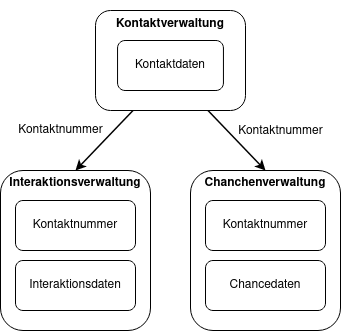
\includegraphics[width=0.65\textwidth]{figures/ContextMap.png}
    \caption{Context Map}
    \label{fig:CRMENTWURF}
\end{figure}

Nachdem die fachliche Einteilung erledigt ist, folgt nun der Entwurf der technischen Architektur. Zur flexiblen Skalierbarkeit müssen die Microservices zustandslos sein. Alle persistenten Daten werden also in einer Datenbank abgelegt. Um eine möglichst große Unabhängigkeit zwischen den Microservices zu haben, wird jedem Microservice eine eigene Datenbank mit einem eigenen Datenbankschema zugeordnet. So können Datenstrukturen geändert werden, ohne unbeabsichtigte Auswirkungen auf andere Microservices zu haben.

Der Interaktions-Microservice und der Chancen-Microservice benötigen für die Zuordnung zu einem Kontakt Informationen vom Kontakt-Microservice. Zwischen diesen Microservices ist somit eine Kommunikation nötig. Gibt es zu viele solcher Abhängigkeiten oder zyklische Aufrufe, sollte die Einteilung der Microservices überarbeitet werden. Das ist bei dieser Aufteilung jedoch nicht der Fall. Da alle Funktionalitäten auch über eine \acp{API} zugänglich sein sollen, bietet es sich an, die Kommunikation zwischen den Microservices auch über diese \acp{API} abzuwickeln.

Um die Microservices klein zu halten wird ein zentrales Frontend entwickelt werden, welches alle Funktionalitäten der Microservices bündelt. Um die Funktionalitäten zu integrieren, greift das Frontend auch auf die \acp{API} der Microservices zu. Somit ergibt sich der folgende Architekturentwurf aus drei verschiedenen Microservices mit drei zugehörigen Datenbanken und einem Frontend.

\begin{figure}[H] 
    \centering
    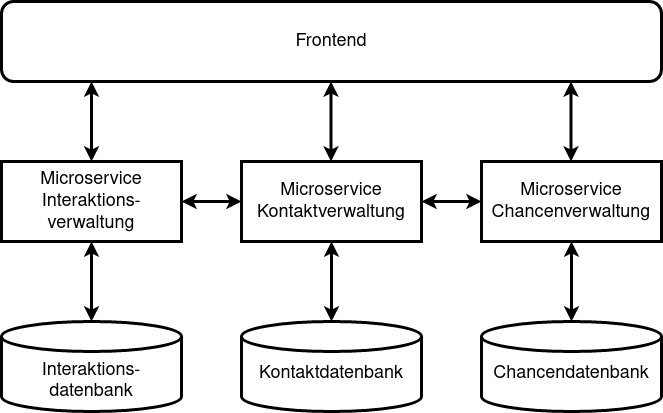
\includegraphics[width=0.8\textwidth]{figures/CRMEntwurf.png}
    \caption{Makro-Architektur des \ac{CRM}-Systems}
    \label{fig:CRMENTWURF}
\end{figure}

Als Nächstes müssen die \acp{API} der Microservices einheitlich spezifiziert werden. Die \ac{API} wird nach dem \ac{REST}-Architekturstil entworfen. Die Kommunikation erfolgt dabei über \ac{HTTP}. Die \ac{REST}-Ressourcen sollen im \ac{JSON}-Format dargestellt werden. Für jeden Microservice werden die Endpunkte unter der die API aufrufbar ist, die HTTP-Anfragemethode und die zu übergebenden Parameter bestimmt.

\begin{figure}[H] 
\centering
    \begin{tabularx}{\columnwidth}[H]{|p{45mm}|p{35mm}|X|}
    		\hline
        \rowcolor{lightgray!20}
        \textbf{Endpunkt} & \textbf{Methode} & \textbf{Beschreibung} \\
        \hline
        \hline
        \multicolumn{3}{|c|}{Microservice Kontaktverwaltung} \\
        \hline
        /contacts & GET & Gibt alle Kontakte zurück \\
        /contacts & POST & Fügt einen neuen Kontakt hinzu \\
        /contacts/\{ID\} & GET & Gibt einen Kontakt zurück \\
        /contacts/\{ID\} & PUT & Ändert einen Kontakt \\
        /contacts/\{ID\} & DELETE & Löscht einen Kontakt \\
        \hline
        \hline
        \multicolumn{3}{|c|}{Microservice Interaktionsverwaltung} \\
        \hline
        /interactions & GET & Gibt alle Interaktionen zurück \\
        /interactions & POST & Fügt einen neue Interaktion hinzu \\
        /interactions/\{ID\} & GET & Gibt eine Interaktion zurück \\
        /interactions/\{ID\} & PUT & Ändert eine Interaktion \\
        /interactions/\{ID\} & DELETE & Löscht eine Interaktion \\
        \hline
        \hline
        \multicolumn{3}{|c|}{Microservice Chancenverwaltung} \\
        \hline
        /opportunity & GET & Gibt alle Chancen zurück \\
        /opportunity & POST & Fügt einen neue Chance hinzu \\
        /opportunity/\{ID\} & GET & Gibt eine Chance zurück \\
        /opportunity/\{ID\} & PUT & Ändert eine Chance \\
        /opportunity/\{ID\} & DELETE & Löscht eine Chance \\
        \hline
    \end{tabularx}
    \caption{Entwurf der REST-API}
\end{figure}

\subsection{Mikro-Architektur}
Für das Gesamtsystem ist die Architektur eines einzelnen Microservice nicht von Bedeutung. Dadurch besitzt man bei der Gestaltung der Mikro-Architektur und vor allem bei der Auswahl des Technologie-Stacks viele Freiheiten. In diesem Fallbeispiel werden bewährte und beliebte Technologien eingesetzt.

Die drei Microservices werden mit demselben Technologie-Stack und einer gleichartigen Architektur entworfen, um den Entwicklungsaufwand zu reduzieren. Es wäre aber auch möglich, alle Microservices mit verschiedenen Technologien zu implementieren, solange sie die gewünschten Schnittstellen anbieten können. Es wird Java in Verbindung mit dem Spring Boot Framework verwendet. Spring Boot bietet ein einsatzfertiges Baugerüst für Java-Anwendungen und eine einfache Auswahl von benötigten Abhängigkeiten, wie beispielsweise Datenbanktreibern. Auch REST-APIs werden von Spring Boot unterstützt. Spring Boot ist auch der De-Facto-Standard für Microservices in Java \parencite[vgl.][]{vmwareinc.Spring2022}.

Für die Datenbanken wird MongoDB verwendet. MongoDB ist ein modernes dokumentorientiertes Datenbankmanagementsystem. Daten werden in Collections als Dokumente mit einem \ac{JSON}-ähnlichen Aufbau verwaltet. Die Datenstrukturen sind flexibel und können leichter umstrukturiert werden als bei klassischen Datenbanken. MongoDB wird auch als NoSQL-Datenbank bezeichnet.

Es werden Domänenmodelle für alle drei Microservices erstellt. Die Domänenmodelle enthalten alle fachlichen Entitäten, deren Eigenschaften und Beziehungen. Für die Modellierung wird ein \acs{UML}-Klassendiagramm verwendet. \ac{UML} ist eine grafische Modellierungssprache, welche noch öfter in dieser Arbeit zum Einsatz kommt. Die Domänenmodelle enhalten die gewünschten Eigenschaften aus den Anforderungen.

Beim Kontakt-Microservice besteht das Datenmodell aus zwei Entitäten. Ein Kontakt besteht aus einer Adresse und mehreren anderen Eigenschaften, wie dem Namen, dem Geburtsdatum und einer Mail-Adresse. Da MongoDB eine NoSQL-Datenbank ist, besitzen die beiden Entitäten keine relationale Beziehung. Die Adresse wird verschachtelt im MongoDB-Dokument vom Kontakt abgespeichert werden. Des Weiteren enthält das Modell zwei Enumerationen für Auswahl des Geschlechts und der Nationalität.

\begin{figure}[H] 
    \centering
    \includegraphics[width=0.9\textwidth]{figures/DomänenmodellKontakt.png}
    \caption{UML-Klassendiagramm als Domänenmodell für den Kontakt-Microservice}
\end{figure} 

Das Datenmodell vom Interaktions-Microservice besteht lediglich aus einer einzelnen Entität und einer Enumeration für die Interaktionsart.

\begin{figure}[H] 
    \centering
    \includegraphics[width=0.9\textwidth]{figures/DomänenmodellInteraktion.png}
    \caption{UML-Klassendiagramm als Domänenmodell für den Interaktions-Microservice}
\end{figure}

Der Chancen-Microservice ist ähnlich aufgebaut und besitzt neben einer einzelnen Entität eine Enumeration für den Status einer Verkaufschance.

\begin{figure}[H] 
    \centering
    \includegraphics[width=0.9\textwidth]{figures/DomänenmodellChance.png}
    \caption{UML-Klassendiagramm als Domänenmodell für den Chancen-Microservice}
\end{figure}

Die einzelnen Microservices werden nach einer hexagonalen Architektur entworfen. Dabei handelt es sich um ein Architekturmuster bei der die Logik im Mittelpunkt steht. Sie hat verschiedene Schnittstellen (Ports), welche mit verschiedenen Adaptern benutzt werden können. Das Architekturmuster wird deshalb auch als Ports und Adapter (Ports and Adapters) bezeichnet. Eine hexagonale Architektur ist eine Weiterentwicklung der klassischen Drei-Schichten-Architektur, bei der eine Anwendung in eine Präsentationsschicht, einen Logikschicht und eine Datenhaltungsschicht aufgeteilt wird.

\begin{figure}[H] 
    \centering
    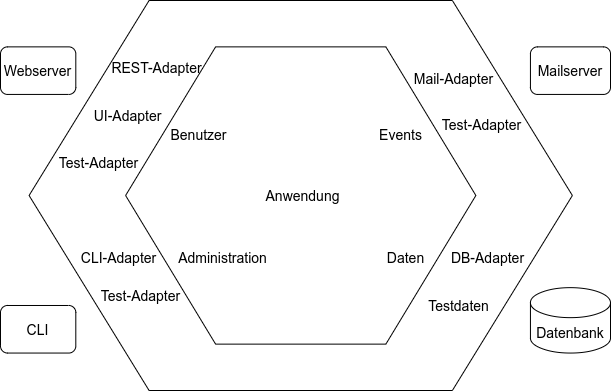
\includegraphics[width=0.9\textwidth]{figures/HexagonalDesignConcept.png}
    \caption{Überblick Hexagonale Architektur \parencite[vgl.][S. 204]{wolffMicroservices2018}}
\end{figure}

Jede Facette der Anwendung, wie Benutzer, Daten oder Admin ist ein Port, welcher von den Adapters Technologien wie REST umgesetzt werden \parencite[vgl.][S. 204]{wolffMicroservices2018}. Die Logik der Anwendung wird klar abgetrennt und nur die Adapter ermöglichen die Kommunikation nach außen. Dadurch bleibt der fachliche Code unabhängig vom technischen Code. Für das Fallbeispiel wird lediglich ein Port für die Daten und ein Port für die Benutzung benötigt. Dazu wird ein Adapter für die REST-API und ein Adapter für MongoDB benötigt.

Für das Frontend wird eine clientseitige Webanwendung eingesetzt. Diese wird mithilfe JavaScript-Bibliothek React verwendet. React ist eine der meistgenutzten Frontend-Bibliotheken.  Anwendungen werden dabei aus wiederverwendbaren Komponenten zusammengesetzt werden, welche effizient gerendert und aktualisiert werden. Die Komponenten können sowohl aus JavaScript, HTML und CSS bestehen.

\clearpage
\section{Implementierung}
In diesem Kapitel wird der erstellte Entwurf implementiert. Zuerst werden die Microservices implementiert und anschließend das Frontend. Es sei auch erwähnt, dass der vollständige Quellcode unter dem folgenden GitHub Repository einsehbar ist: \href{https://github.com/SimonHirner/bachelor-thesis}{github.com/SimonHirner/bachelor-thesis}.

Darüber hinaus wird Swagger in die Microservices integriert. Bei Swagger handelt es sich ein Werkzeug zur sprachunabhängigen Spezifikation von APIs. Swagger kann durch eine Abhängigkeit zu Spring Boot hinzu gefügt werden. Es erstellt automatisch eine Webseite mit der Dokumentation unserer API. Um das Monitoring, Service Discovery, Load Balancing wird mit Kubernetes gelöst. Unser System muss diese Aufgaben also nicht selbst bewältigen und diese Bestandteile werden erst in der Bereitstellung konfiguriert.

\subsection{Microservices}
Die Umsetzung aller drei Microservices ist sehr ähnlich, deshalb wird die Implementierung hauptsächlich am Beispiel des Kontakt-Microservices erläutert. Als Erstes wird das erstellte Domänenmodelle für den Kontakt-Microservice umgesetzt. Jede Entität wird mit seinen Eigenschaften als eine Klasse mit Attributen in Java implementiert. Die Endpunkte unserer spezifizierten REST-API werden in der Klasse ContactController erstellt. Dieser fungiert als ein Adapter im Sinne der hexagonalen Architektur. Er benötigt einen Port, mit dem er auf Funktionen der Geschäftslogik zugreifen kann. Dafür wird das Interface ContactService erstellt. Dieses definiert die Funktionalitäten der Geschäftslogik, implementiert sie aber noch nicht. Erst in der Klasse ContactServiceImpl wird das Interface implementiert und die eigentliche Geschäftslogik programmiert. Dadurch ist die Logik vom Controller, der sich um die Anfragen auf die REST-Schnittstelle kümmert, unabhängig. Einen Adapter für die Anbindung an MongoDB bringt Spring bereits mit. Es muss lediglich noch das Interface ContactRepository erstellt werden, welcher als Port den Adapter mit der Geschäftslogik verbindet.

\begin{lstlisting}[language=java, caption=Dockerfile für Frontend]
@GetMapping("/{id}")
@ApiOperation(value = "Get Contact by ID.")
Contact getContact(@PathVariable String id) {
    return contactService.getContact(id)
            .orElseThrow(() -> new ResourceNotFoundException(id));
}
\end{lstlisting}

\begin{lstlisting}[language=java, caption=Dockerfile für Frontend]
@Override
public Optional<Contact> getContact(String id) {
   return contactRepository.findById(id);
}
\end{lstlisting}

\begin{figure}[H] 
    \centering
    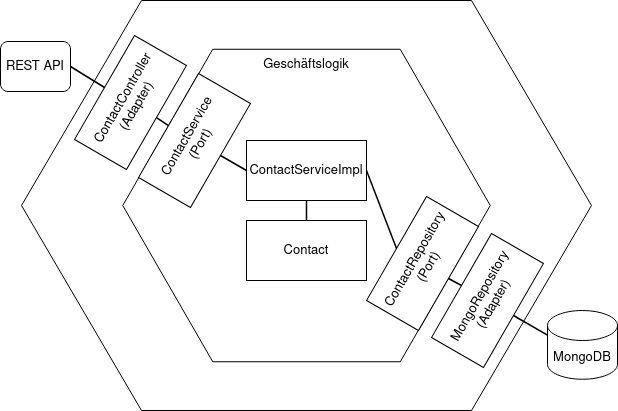
\includegraphics[width=0.9\textwidth]{figures/HexagonalDesign.png}
    \caption{Implementierung der hexagonalen Architektur}
\end{figure}

Den Mittelpunkt bildet die Klasse ContactServiceImpl. Sie enthählt den Code, der die Geschäftslogik, beschreibt. Die Klasse enthält verschiedene Methoden, um Kontakte zurückzugeben, zu löschen, zu speichern und zu ersetzen.

\begin{figure}[H] 
    \centering
    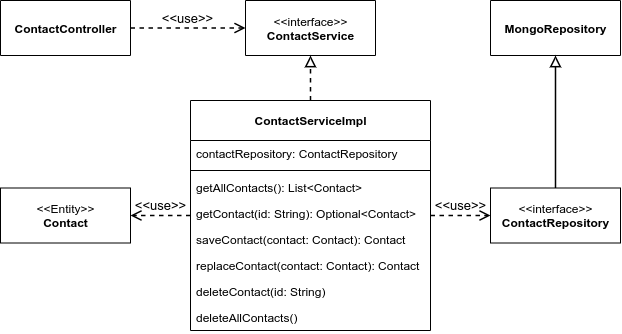
\includegraphics[width=0.9\textwidth]{figures/UMLKlassenDiagrammKontakt.png}
    \caption{Entwurf des}
\end{figure}

Der Interaktions-Microservice und der Chancen-Microservices unterscheiden sich bei der Geschäftslogik vom Kontakt-Microservice. Der Interaktions-Microservice muss nämlich beim Speichern einer Interaktion überprüfen, ob die Kontaktidentifikationsnummer der Interaktion gültig ist. Dafür ruft der Interaktions-Microservice den Kontakt-Microservice über die REST-API auf und testet, ob zu der angegebenen Kontaktidentifikationsnummer ein Kontakt vorhanden ist. Da bei einer Chance auch eine Kontaktidentifikationsnummer angegeben wird, wird hier auch der Kontakt-Microservice aufgerufen.

\begin{figure}[H] 
    \centering
    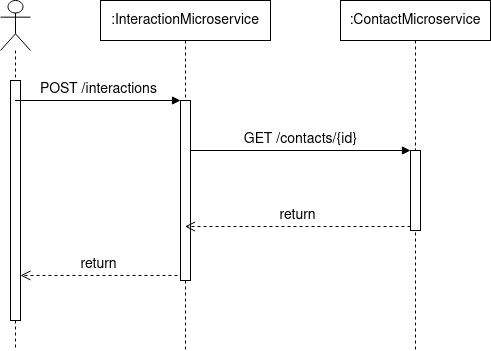
\includegraphics[width=0.75\textwidth]{figures/UMLSequenzdiagramm.png}
    \caption{UML-Sequenzdiagramm}
\end{figure}



Alle drei Microservices benötigen die \ac{URI} ihrer Datenbank, um mit ihr eine Verbindung aufzubauen. Der Interaktions-Microservice und der Verkaufschancen-Microservice brauchen darüber hinaus die Adresse des Kontakt-Microservices, um mit diesem zu Kommunizieren. Diese Verbindungsinformationen, werden den Anwendungen über Umgebungsvariablen übergeben. Später bei der Bereitstellung, kann mit Kubernetes den Containern die passenden Umgebungsvariablen so übergeben werden.

\subsection{Frontend}

Das Frontend. Das Frontend soll später auch mit Kubernetes bereitgestellt werden, es wird aber nicht als Microservices angesehen. Das Frontend benötigt die \ac{URI} aller Services. Auch hier werden die Verbindungsinformationen über eine Umgebungsvariable übergeben.

\clearpage
\section{Bereitstellung mit Kubernetes}

Im letzten Teil des Fallbeispiels wird das fertige CRM-System nun mit Kubernetes bereitgestellt.

\subsection{Containerisierung}

Um die Microservices und das Frontend in Pods in einem Kubernetes Cluster laufen zu lassen, müssen sie erst mit Docker containerisiert werden. Dazu wird als Erstes ein Dockerfile für jeden Microservice erstellt. Anschließend kann aus dem Dockerfile ein Docker Image gebaut werden, mit dem dann ein entsprechender Container gestartet werden kann.

Dockerfiles besitzen eine eigene Syntax. Ein großgeschriebener Befehl wird gefolgt von einem oder mehreren Parametern. Es ist aufgebaut wie eine Anleitung, welche Schritt für Schritt abgearbeitet wird. Die Dockerfiles der Microservices haben alle den selben Aufbau, da alle drei Projekte auch die selben Aufbau und die selben Technologien verwenden. Der erste Befehl in den Dockerfiles bestimmt, auf welchem Docker Image unser eigenes Image basieren soll. Hier wird ein Image mit einer Java-Plattform verwendet, welches automatisch aus dem öffentlichen DockerHub heruntergeladen wird. Anschließend wird die JAR-Datei der Anwendung in das Image kopiert. Als letzter Befehl wird festgelegt, dass die JAR-Datei beim Start des Containers ausgeführt werden soll.

\begin{lstlisting}[language=dockerfile, caption=Dockerfile für Kontakt-Microservice]
FROM openjdk:11-jdk-slim
ARG JAR_FILE=target/*.jar
COPY ${JAR_FILE} app.jar
EXPOSE 8080
ENTRYPOINT ["java","-jar","/app.jar"]
\end{lstlisting}

Das Frontend benötigt ein eigenes Dockerfile. Dieses hat einen mehrstufigen Aufbau. Im ersten Stufe, der Build-Stage, wird unsere React-Anwendung gebaut. Um die fertig gebaute Webanwendung an einen Browser auszuliefern wird ein Webserver benötigt. In der zweiten Stufe des Dockerfiles basiert auf einem Image mit dem Webserver Nginx. Die React-Anwendung aus der Build-Stage wird nun in das finale Image kopiert.

\begin{lstlisting}[language=dockerfile, caption=Dockerfile für Frontend]
FROM node:alpine as build
WORKDIR /app
COPY package*.json ./
RUN npm install --silent
COPY . .
RUN npm run build

FROM nginx:alpine
WORKDIR /usr/share/nginx/html
RUN rm -rf ./*
COPY --from=build /app/build .
ENTRYPOINT ["nginx", "-g", "daemon off;"]
\end{lstlisting}

Für die Datenbanken müssen keine eigenen Dockerfiles erstellt werden. Hier reichen unveränderte Images, welche aus dem DockerHub heruntergeladen werden können, aus. Mit dem folgenden Befehl kann aus dem Dockerfile nun ein Docker Image gebaut werden.

\begin{lstlisting}[language=bash, caption=Befehl , captionpos=b]
docker build -t contact-microservice:latest .
\end{lstlisting}


\subsection{Bereitstellung}

Für jede Datenbank wird eine Anwendung 

\begin{figure}[H] 
    \centering
    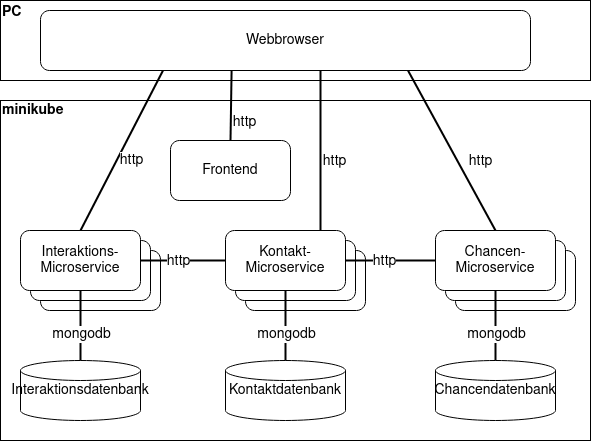
\includegraphics[width=0.71\textwidth]{figures/DeploymentDiagramm.png}
    \caption{Entwurf des \acp{Hexagonale Architektur}}
    \label{fig:CRMENTWURF}
\end{figure}

Jetzt müssen die fertigen Images in unserem Kubernetes Cluster bereitgestellt werden. Dafür werden YAML-Dateien erstellt, in denen die gewünschten Kubernetes Objekte beschrieben werden. Für jeden der drei Microservices und das Frontend muss ein Service und ein Deployment erstellt werden. Das Deployment repräsentiert die Anwendung. Mit Parametern kann festgelegt werden wie viele Pods mit der Anwendung gestartet werden sollen.

\begin{lstlisting}[language=YAML, caption=Befehl]
apiVersion: apps/v1
kind: Deployment
metadata:
  name: contact-service
spec:
  replicas: 1
  template:
    metadata:
      labels:
        app: contact-service
    spec:
      containers:
        - name: contact-service
          image: contact-microservice:latest
          imagePullPolicy: IfNotPresent
          ports:
          - containerPort: 8080
          env:
            - name: MONGODB_HOST
              valueFrom:
                configMapKeyRef:
                  name: contact-db-config  
                  key: host
\end{lstlisting}

\begin{lstlisting}[language=YAML, morekeywords=host, caption=Befehl , captionpos=b]
apiVersion: v1
kind: ConfigMap
metadata:
   name: contact-service-config
data:
 host: contact-service
\end{lstlisting}

Nach der Erstellung der Services wird die Service Discovery und Lasterverteilung von Kubernetes übernommen. 

\begin{lstlisting}[language=YAML, caption=Befehl , captionpos=b]
kind: Service
apiVersion: v1
metadata:
  name: contact-service
spec:
  selector:
    app: contact-service
  ports:
  - protocol: TCP
    port: 8080
    nodePort: 30010
  type: NodePort
\end{lstlisting}

Nun müssen nur noch alle YAML-Dateien über den folgenden kubectl-Befehl angewendet werden. Kubernetes sorg nun dafür, dass die beschriebenen Objekte, erstellt werden.

\begin{lstlisting}[language=bash, caption=Befehl , captionpos=b]
kubectl apply -f contact-microservice.yaml
\end{lstlisting}

\subsection{Skalierung}

Um die Vorteile von unseren Microservices auszunutzen, sollen die Microservices nun horizontal skaliert werden. Auch dafür wird eine YAML-Datei erstellt, in der ein HorizontalPodAutoscaler-Objekt für jeden Microservice beschrieben wird. In der Datei wird angegeben, welches Deployment skaliert werden soll. Als Metrik, wann hochskaliert werden soll, kann die CPU-Auslastung des Pods verwendet werden. Darüber hinaus wird angegeben wie viele Pods von dem entsprechenden Microservice minimal und maximal ausgeführt werden sollen.

\begin{lstlisting}[language=YAML, caption=Befehl , captionpos=b]
apiVersion: autoscaling/v1
kind: HorizontalPodAutoscaler
metadata:
    name: contact-service
spec:
    scaleTargetRef:
        apiVersion: apps/v1
        kind: Deployment
        name: contact-service
    minReplicas: 2
    maxReplicas: 4
    targetCPUUtilizationPercentage: 80
\end{lstlisting}
